\subsection{Bau der Mechanik}
Beim Bau der Mechanik wurde großteils nach dem, zuvor im Zuge der Konstruktionsplanung erstellten, 3D Modell vorgegangen. Das Material für das Modell wurde beinahe ausschließlich aus 2,5 cm dicken Dreischichtplatten gewonnen, als Wellenverlängerungen für die Motoren dienen Alurohre mit einem Durchmesser von 10 mm. 
Beim Bau des Roboters wurde in folgenden Schritten vorgegangen:
\begin{itemize}
\item \textbf{Zuschneiden einer Grundplatte und Anbringung der Basis}\\
Der Erste Schritt beim Bau des Modells war das grobe Zuschneiden der Grundplatte, welche später die gesamte Arbeitsfläche des Armes abdecken sollte und die Stabilität des Arms gewährleistet.
Direkt auf diese Grundplatte wurde dann die Basis des Roboters geschraubt. Bei der Basis handelt es sich um eine senkrecht aufgestellte Platte, an der später die Halterung für die primäre Achse befestigt wurde.

\item \textbf{Bau des ersten Gelenks}\\
Das erste Gelenk des  Edubot Modells wurde direkt mit der Basis verschraubt und bietet damit einen sehr hohen Grad an Stabilität. Grundsätzlich basiert das Gelenk auf der Form eines liegenden U welches über zwei Kugellager eine etwa 1 cm dicke Verlängerung der Motorwelle aus Aluminium hält. An diese Verlängerung ist in weiterer Folge die primäre Achse des Motors so festgeklemmt, so dass sie im 90$^\circ$ Winkel zur senkrecht stehenden Wellenverlängerung steht.

\begin{figure}[H]
\centering
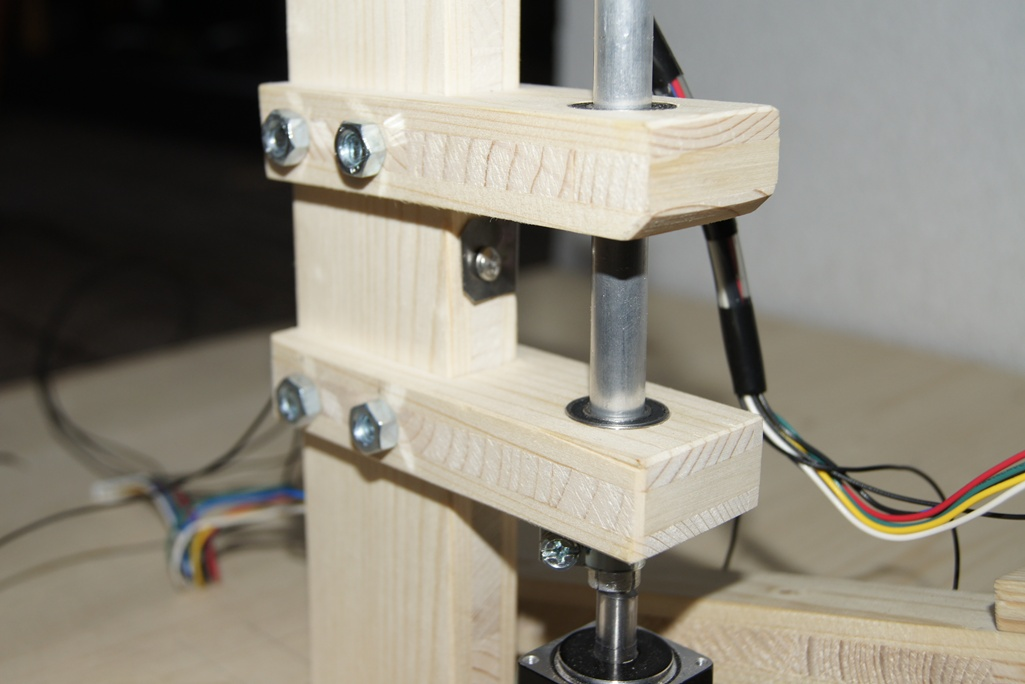
\includegraphics[width=11cm]{images/gelenk_photo}
\caption{Das erste Gelenke (ohne Achse)}
\end{figure}

\item \textbf{Befestigung des ersten Arms}\\
Für das Anklemmen der Achse an die Wellenverlängerung wurde der erste Arm mit einer 1 cm dicken Bohrung versehen durch welche die Wellenverlängerung exakt passt. Zusätzlich wurde die Achse der Länge nach durch die Mitte des Lochs etwa 4 cm eingeschnitten. Durch das spätere anbringen von Schrauben (entsprechende Bohrungen waren zuvor nötig), die den entstandenen Spalt zusammenziehen können, wurde es möglich das gebohrte Loch nach durchstecken der Wellenverlängerung zusätzlich zu verkleinern und somit die Achse fest einzuklemmen.
\begin{figure}[H]
\centering
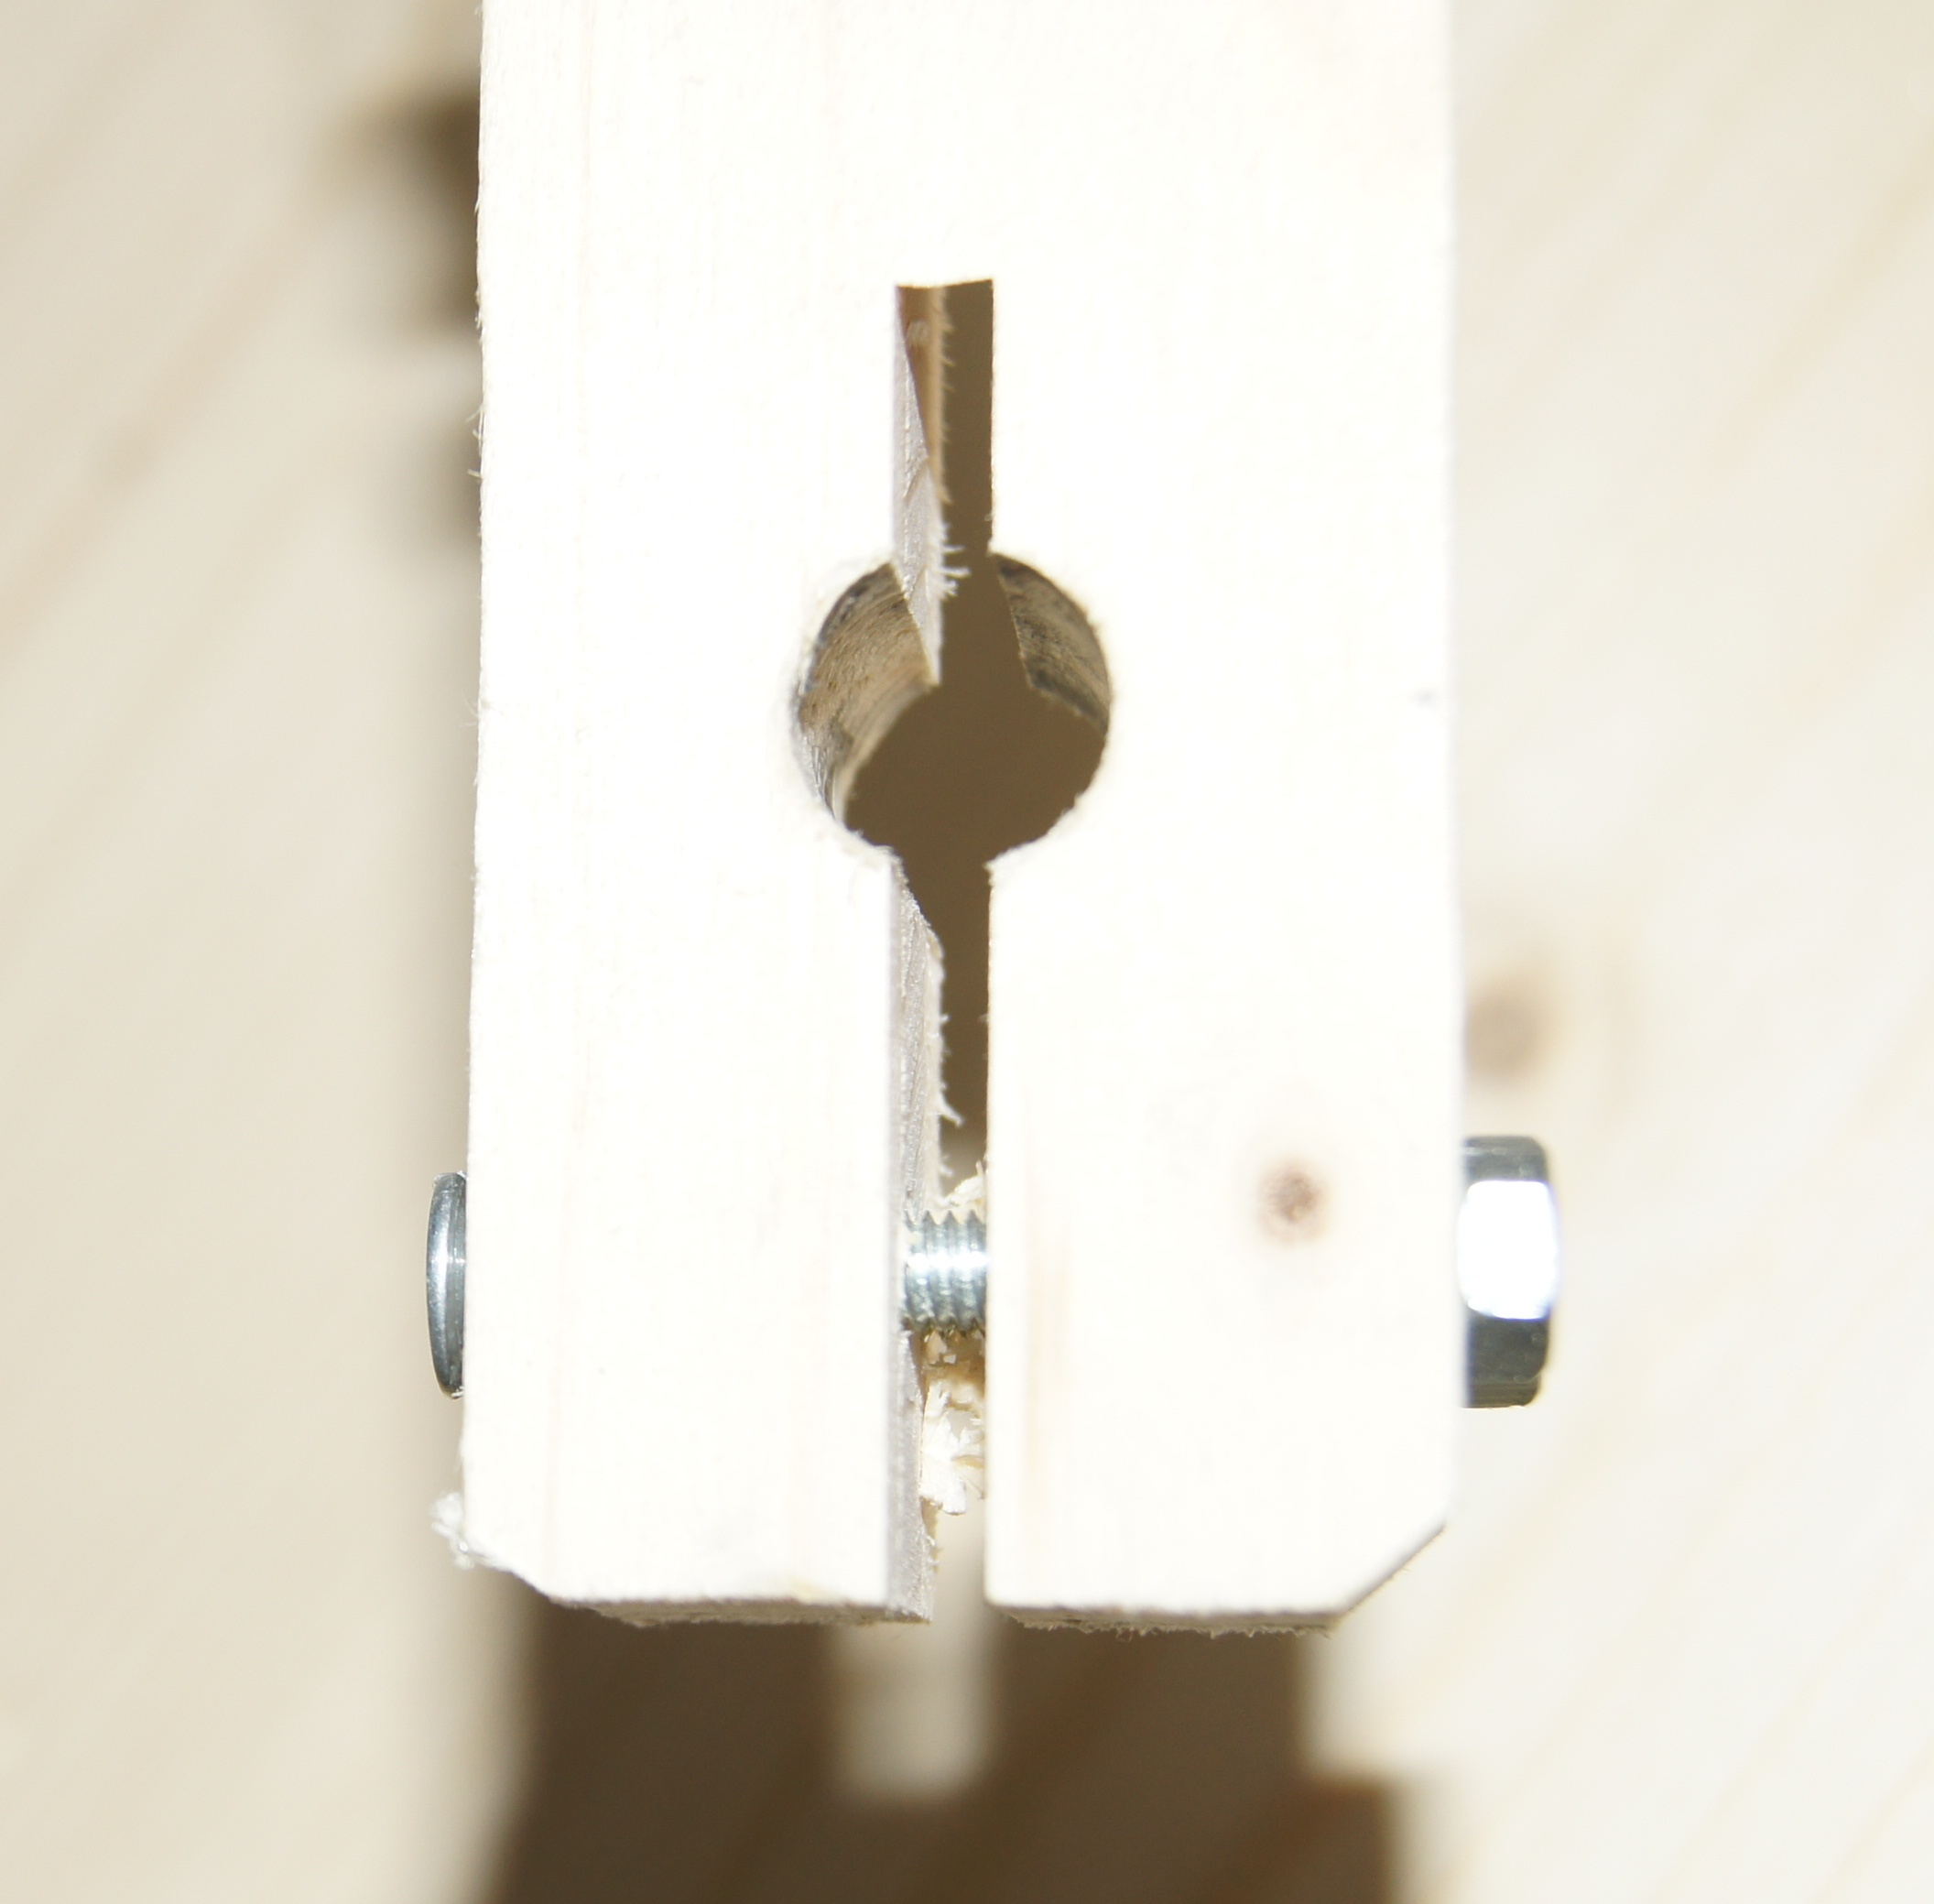
\includegraphics[width=8cm]{images/axis_fix}
\caption{Der Klemmmechanismus der Achse}
\end{figure}

Der erste Arm (primäre Achse) hat eine Länge von 20 cm.
\item \textbf{Bau des zweiten Gelenks}\\
Das zweite Gelenk wurde an direkt mit der primären Achse verschraubt und basiert wieder auf dem selben Prinzip wie das erste Gelenk. Beim Bau des zweiten Gelenks ergaben sich zwei kleine Unterschiede gegenüber dem großen Gelenk. Der erste Unterschied ist, dass das zweite Gelenk kleiner ist und aus Gewichtsgründen der Fokus nicht nur auf der Stabilität der Konstruktion lag. 
Der zweite Unterschied ist die Positionierung der Achse. Beim ersten Gelenk wurde die Achse zwischen den beiden Kugellagern, in der Mitte der U-Förmigen Konstruktion angebracht, beim zweiten Gelenk wurde die Achse unterhalb des Us angebracht. Diese Abänderung der ursprünglichen Konstruktion führt nur zu einem geringen Verlust an Stabilität und erweitert im Gegenzug den Arbeitsbereich des Roboters.
\item \textbf{Befestigung des zweiten Armes}\\
Bei der Befestigung des zweiten Armes (sekundär Achse) wurde im Prinzip gleich vorgegangen wie beim ersten Arm (primär Achse), für eine genauere Beschreibung siehe den Punkt "Befestigung der ersten Achse" weiter oben in dieser Aufzählung.
\item \textbf{Befestigung der Motoren}\\
Der Motor der primären Achse wurde direkt mit der Grundplatte des Motors verschraubt und läuft damit wenig Gefahr durch Verwindung oder Verrutschen die Positionierung des Arms zu verfälschen.
Der Motor der sekundären Achse wurde an das zweite Gelenk geschraubt, welches seinerseits direkt mit der primären Achse verbunden ist. Durch die Positionierung des zweiten Motors ohne zusätzlichen Abstand direkt über dem zweiten Gelenk war es möglich die Verbindung mit der Wellenverlängerung direkt im Gelenk herzustellen und damit auf eine komplexere Konstruktion zu verzichten. Die folgende Grafik zeigt am Beispiel des ersten Motors, wie die Verbindung der Motorwelle mit der Wellenverlängerung gelöst wurde
\end{itemize}
\subsubsection{Planung und Bau der Elektronik}
Die Planung der Elektronik war ein stetiger Prozess und ging einher mit dem versuchsweisen Aufbau der jeweiligen Planungsergebnisse. Grob unterteilen lässt sich die Entwicklung jedoch in drei Phasen:
\begin{itemize}
\item \textbf{Versuchsweiser Aufbau mit direkter Ansteuerung}\\
In einem ersten Anlauf wurde der Versuch unternommen, die gesamte Ansteuerung der Schrittmotorsteuerungen und damit auch deren Versorgung mit dem Entsprechenden Taktsignal das zum Verfahren der Schritte benötigt wird, über ein USB Modul für den PC zu realisieren. Der Vorteil dieser Variante wäre gewesen, dass eine solche Ansteuerung aus softwaretechnischer Sicht wesentlich leichter zu realisieren gewesen wäre. Nach einigen Versuchen mit diesem Aufbau stellte sich jedoch heraus, dass aufgrund mangelnder Echtzeitqualitäten von Microsoft Windows die Ausgabe des sehr hochfrequenten Taktsignals nicht stabil möglich ist.
\item \textbf{Versuchsweiser Aufbau mit Mikrocontroller Steuerung}\\
Auf Basis der gewonnenen Erfahrungen aus dem Aufbau mit dem USB Modul, wurde nun überlegt wie das Taktsignal stabilisiert werden könnte und wie eine Ausgabe mit höherer Frequenz möglich werden würde. Es wurde schließlich beschlossen, die Ausgabe des Taktsignals, sowie sämtliche direkt mit der Elektronik des Roboters zusammenhängende Aufgaben von einem Mikrocontroller übernehmen zu lassen. Der Mikrocontroller wird über die Netzwerkschnittstelle mit Daten über die Verfahrbewegung versorgt und kann schließlich die Elektronik des Roboters autonom steuern.
\item \textbf{Endaufbau am Modell mit Endschaltern}\\
Nach Fertigstellung des Holzmodells wurde der zuerst nur versuchsweise Aufbau der oben Beschriebenen Variante mit Mikrocontroller in das Modell eingebaut. In diesem Schritt wurden nun auch die Schalter für den "'Homing Prozess"', in Form einfacher Kontaktflächen, eingebaut und mit dem Mikrocontroller verbunden.
\begin{figure}[H]
\centering
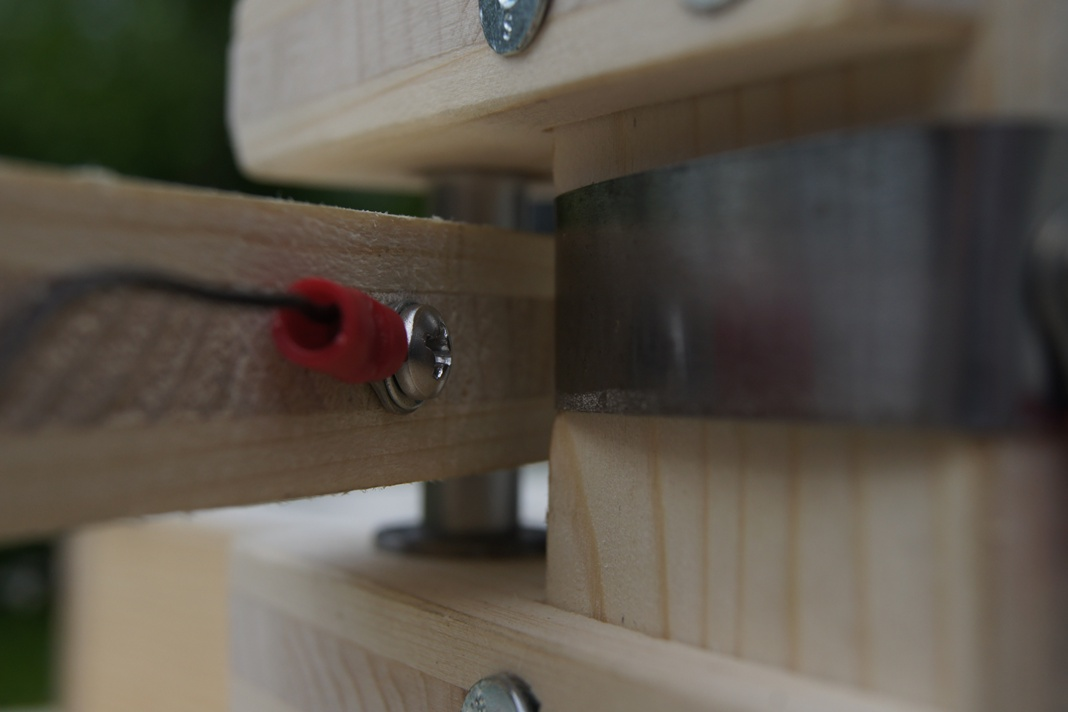
\includegraphics[width=11cm]{images/contact}
\caption{Die Kontaktstelle für die primäre Achse}
\end{figure}

Zum Schluss war es noch nötig, die endgültige Schaltung zu Verlöten und durch den Einsatz eines Spannungsteilers das Labornetzteil zu ersetzen.
\end{itemize}

Nähere Informationen zu Aufbau und Funktionsweise der Elektronik sind dem Kapitel "'Elektronik"' zu entnehmen.